% Options for packages loaded elsewhere
\PassOptionsToPackage{unicode}{hyperref}
\PassOptionsToPackage{hyphens}{url}
%
\documentclass[
  man,floatsintext]{apa6}
\usepackage{amsmath,amssymb}
\usepackage{lmodern}
\usepackage{iftex}
\ifPDFTeX
  \usepackage[T1]{fontenc}
  \usepackage[utf8]{inputenc}
  \usepackage{textcomp} % provide euro and other symbols
\else % if luatex or xetex
  \usepackage{unicode-math}
  \defaultfontfeatures{Scale=MatchLowercase}
  \defaultfontfeatures[\rmfamily]{Ligatures=TeX,Scale=1}
\fi
% Use upquote if available, for straight quotes in verbatim environments
\IfFileExists{upquote.sty}{\usepackage{upquote}}{}
\IfFileExists{microtype.sty}{% use microtype if available
  \usepackage[]{microtype}
  \UseMicrotypeSet[protrusion]{basicmath} % disable protrusion for tt fonts
}{}
\makeatletter
\@ifundefined{KOMAClassName}{% if non-KOMA class
  \IfFileExists{parskip.sty}{%
    \usepackage{parskip}
  }{% else
    \setlength{\parindent}{0pt}
    \setlength{\parskip}{6pt plus 2pt minus 1pt}}
}{% if KOMA class
  \KOMAoptions{parskip=half}}
\makeatother
\usepackage{xcolor}
\usepackage{graphicx}
\makeatletter
\def\maxwidth{\ifdim\Gin@nat@width>\linewidth\linewidth\else\Gin@nat@width\fi}
\def\maxheight{\ifdim\Gin@nat@height>\textheight\textheight\else\Gin@nat@height\fi}
\makeatother
% Scale images if necessary, so that they will not overflow the page
% margins by default, and it is still possible to overwrite the defaults
% using explicit options in \includegraphics[width, height, ...]{}
\setkeys{Gin}{width=\maxwidth,height=\maxheight,keepaspectratio}
% Set default figure placement to htbp
\makeatletter
\def\fps@figure{htbp}
\makeatother
\setlength{\emergencystretch}{3em} % prevent overfull lines
\providecommand{\tightlist}{%
  \setlength{\itemsep}{0pt}\setlength{\parskip}{0pt}}
\setcounter{secnumdepth}{-\maxdimen} % remove section numbering
% Make \paragraph and \subparagraph free-standing
\ifx\paragraph\undefined\else
  \let\oldparagraph\paragraph
  \renewcommand{\paragraph}[1]{\oldparagraph{#1}\mbox{}}
\fi
\ifx\subparagraph\undefined\else
  \let\oldsubparagraph\subparagraph
  \renewcommand{\subparagraph}[1]{\oldsubparagraph{#1}\mbox{}}
\fi
\newlength{\cslhangindent}
\setlength{\cslhangindent}{1.5em}
\newlength{\csllabelwidth}
\setlength{\csllabelwidth}{3em}
\newlength{\cslentryspacingunit} % times entry-spacing
\setlength{\cslentryspacingunit}{\parskip}
\newenvironment{CSLReferences}[2] % #1 hanging-ident, #2 entry spacing
 {% don't indent paragraphs
  \setlength{\parindent}{0pt}
  % turn on hanging indent if param 1 is 1
  \ifodd #1
  \let\oldpar\par
  \def\par{\hangindent=\cslhangindent\oldpar}
  \fi
  % set entry spacing
  \setlength{\parskip}{#2\cslentryspacingunit}
 }%
 {}
\usepackage{calc}
\newcommand{\CSLBlock}[1]{#1\hfill\break}
\newcommand{\CSLLeftMargin}[1]{\parbox[t]{\csllabelwidth}{#1}}
\newcommand{\CSLRightInline}[1]{\parbox[t]{\linewidth - \csllabelwidth}{#1}\break}
\newcommand{\CSLIndent}[1]{\hspace{\cslhangindent}#1}
\ifLuaTeX
\usepackage[bidi=basic]{babel}
\else
\usepackage[bidi=default]{babel}
\fi
\babelprovide[main,import]{english}
% get rid of language-specific shorthands (see #6817):
\let\LanguageShortHands\languageshorthands
\def\languageshorthands#1{}
% Manuscript styling
\usepackage{upgreek}
\captionsetup{font=singlespacing,justification=justified}

% Table formatting
\usepackage{longtable}
\usepackage{lscape}
% \usepackage[counterclockwise]{rotating}   % Landscape page setup for large tables
\usepackage{multirow}		% Table styling
\usepackage{tabularx}		% Control Column width
\usepackage[flushleft]{threeparttable}	% Allows for three part tables with a specified notes section
\usepackage{threeparttablex}            % Lets threeparttable work with longtable

% Create new environments so endfloat can handle them
% \newenvironment{ltable}
%   {\begin{landscape}\centering\begin{threeparttable}}
%   {\end{threeparttable}\end{landscape}}
\newenvironment{lltable}{\begin{landscape}\centering\begin{ThreePartTable}}{\end{ThreePartTable}\end{landscape}}

% Enables adjusting longtable caption width to table width
% Solution found at http://golatex.de/longtable-mit-caption-so-breit-wie-die-tabelle-t15767.html
\makeatletter
\newcommand\LastLTentrywidth{1em}
\newlength\longtablewidth
\setlength{\longtablewidth}{1in}
\newcommand{\getlongtablewidth}{\begingroup \ifcsname LT@\roman{LT@tables}\endcsname \global\longtablewidth=0pt \renewcommand{\LT@entry}[2]{\global\advance\longtablewidth by ##2\relax\gdef\LastLTentrywidth{##2}}\@nameuse{LT@\roman{LT@tables}} \fi \endgroup}

% \setlength{\parindent}{0.5in}
% \setlength{\parskip}{0pt plus 0pt minus 0pt}

% Overwrite redefinition of paragraph and subparagraph by the default LaTeX template
% See https://github.com/crsh/papaja/issues/292
\makeatletter
\renewcommand{\paragraph}{\@startsection{paragraph}{4}{\parindent}%
  {0\baselineskip \@plus 0.2ex \@minus 0.2ex}%
  {-1em}%
  {\normalfont\normalsize\bfseries\itshape\typesectitle}}

\renewcommand{\subparagraph}[1]{\@startsection{subparagraph}{5}{1em}%
  {0\baselineskip \@plus 0.2ex \@minus 0.2ex}%
  {-\z@\relax}%
  {\normalfont\normalsize\itshape\hspace{\parindent}{#1}\textit{\addperi}}{\relax}}
\makeatother

% \usepackage{etoolbox}
\makeatletter
\patchcmd{\HyOrg@maketitle}
  {\section{\normalfont\normalsize\abstractname}}
  {\section*{\normalfont\normalsize\abstractname}}
  {}{\typeout{Failed to patch abstract.}}
\patchcmd{\HyOrg@maketitle}
  {\section{\protect\normalfont{\@title}}}
  {\section*{\protect\normalfont{\@title}}}
  {}{\typeout{Failed to patch title.}}
\makeatother

\usepackage{xpatch}
\makeatletter
\xapptocmd\appendix
  {\xapptocmd\section
    {\addcontentsline{toc}{section}{\appendixname\ifoneappendix\else~\theappendix\fi\\: #1}}
    {}{\InnerPatchFailed}%
  }
{}{\PatchFailed}
\keywords{visual illusions, illusion game, pyllusion, illusion effect, personality\newline\indent Word count: 1156}
\usepackage{lineno}

\linenumbers
\usepackage{csquotes}
\usepackage[titles]{tocloft}
\cftpagenumbersoff{figure}
\renewcommand{\cftfigpresnum}{\itshape\figurename\enspace}
\renewcommand{\cftfigaftersnum}{.\space}
\setlength{\cftfigindent}{0pt}
\setlength{\cftafterloftitleskip}{0pt}
\settowidth{\cftfignumwidth}{Figure 10.\qquad}
\usepackage[labelfont=bf, font={scriptsize, color=gray}]{caption}
\ifLuaTeX
  \usepackage{selnolig}  % disable illegal ligatures
\fi
\IfFileExists{bookmark.sty}{\usepackage{bookmark}}{\usepackage{hyperref}}
\IfFileExists{xurl.sty}{\usepackage{xurl}}{} % add URL line breaks if available
\urlstyle{same} % disable monospaced font for URLs
\hypersetup{
  pdftitle={The Illusion Game: A Novel Experimental Paradigm Provides Evidence in Favour of a General Factor of Visual Illusion Sensitivity and Personality Correlates},
  pdfauthor={Dominique Makowski1},
  pdflang={en-EN},
  pdfkeywords={visual illusions, illusion game, pyllusion, illusion effect, personality},
  hidelinks,
  pdfcreator={LaTeX via pandoc}}

\title{\textbf{The Illusion Game: A Novel Experimental Paradigm Provides Evidence in Favour of a General Factor of Visual Illusion Sensitivity and Personality Correlates}}
\author{Dominique Makowski\textsuperscript{1}}
\date{}


\shorttitle{Illusion Game}

\authornote{

Correspondence concerning this article should be addressed to Dominique Makowski, HSS 04-18, 48 Nanyang Avenue, Singapore (\href{mailto:dom.makowski@gmail.com}{\nolinkurl{dom.makowski@gmail.com}}).

Correspondence concerning this article should be addressed to Dominique Makowski, HSS 04-18, 48 Nanyang Avenue, Singapore. E-mail: \href{mailto:dom.makowski@gmail.com}{\nolinkurl{dom.makowski@gmail.com}}

}

\affiliation{\vspace{0.5cm}\textsuperscript{1} School of Social Sciences, Nanyang Technological University, Singapore}

\abstract{%
Abstract abstract. We invite researchers to re-analyze our open-access data to provide complimentary evidence (or absence thereof) on the effect and structure of illusion sensitivity.
}



\begin{document}
\maketitle

\hypertarget{introduction}{%
\section{Introduction}\label{introduction}}

Visual illusions are fascinating stimuli, capturing a key feature of our neurocognitive systems.
They eloquently show that our brains did not evolve to be perfect perceptual devices providing veridical accounts of physical reality, but to integrate prior knowledge and contextual information - blended together in our subjective conscious experience (Carbon, 2014).
Despite the historical and intensive interest within the fields of visual perception (Day, 1972; Eagleman, 2001; Gomez-Villa et al., 2022), consciousness science (Caporuscio et al., 2022; Lamme, 2020), and psychiatry (Gori et al., 2016; Notredame et al., 2014; Razeghi et al., 2022; Teufel et al., 2015), several important issues remain open.

Notably, the presence of a common mechanism underlying the effect of different illusions has been contested (Cretenoud et al., 2020, 2019a; Hamburger, 2016; Teufel et al., 2018b); and the nature of the underlying processes - whether related to low-level features of the visual processing system (Cretenoud et al., 2019b; Gori et al., 2016) or to top-down influences of prior beliefs (Caporuscio et al., 2022; Teufel et al., 2018a) are strongly debated. The existence of dispositional correlates of illusion sensitivity - for example, higher illusion resistance has been reported in schizophrenia and autism (Giaouri \& Alevriadou, 2011; Keane et al., 2014; Notredame et al., 2014; Park et al., 2022) or \textbf{Insert some demographic / personality feature} {[}\textbf{REF}{]} - is another area of controversy.

One key challenge hindering the further development of illusion research is the relative difficulty in adapting visual illusions to an experimental setting, which typically requires the controlled modulation of the specific variables of interest.
To address this issue, we first developed a parametric framework to manipulate visual illusions, which we implemented and made accessible in the open-source software \emph{Pyllusion} (Makowski et al., 2021a).
This software allows us to generate different types of classic visual illusions (e.g., Müller-Lyer, Ponzo, Delboeuf, Ebbinghaus) with a continuous and independent modulation of two parameters: \emph{illusion strength} and \emph{task difficulty} (see \textbf{Figure 1}).

\begin{figure}
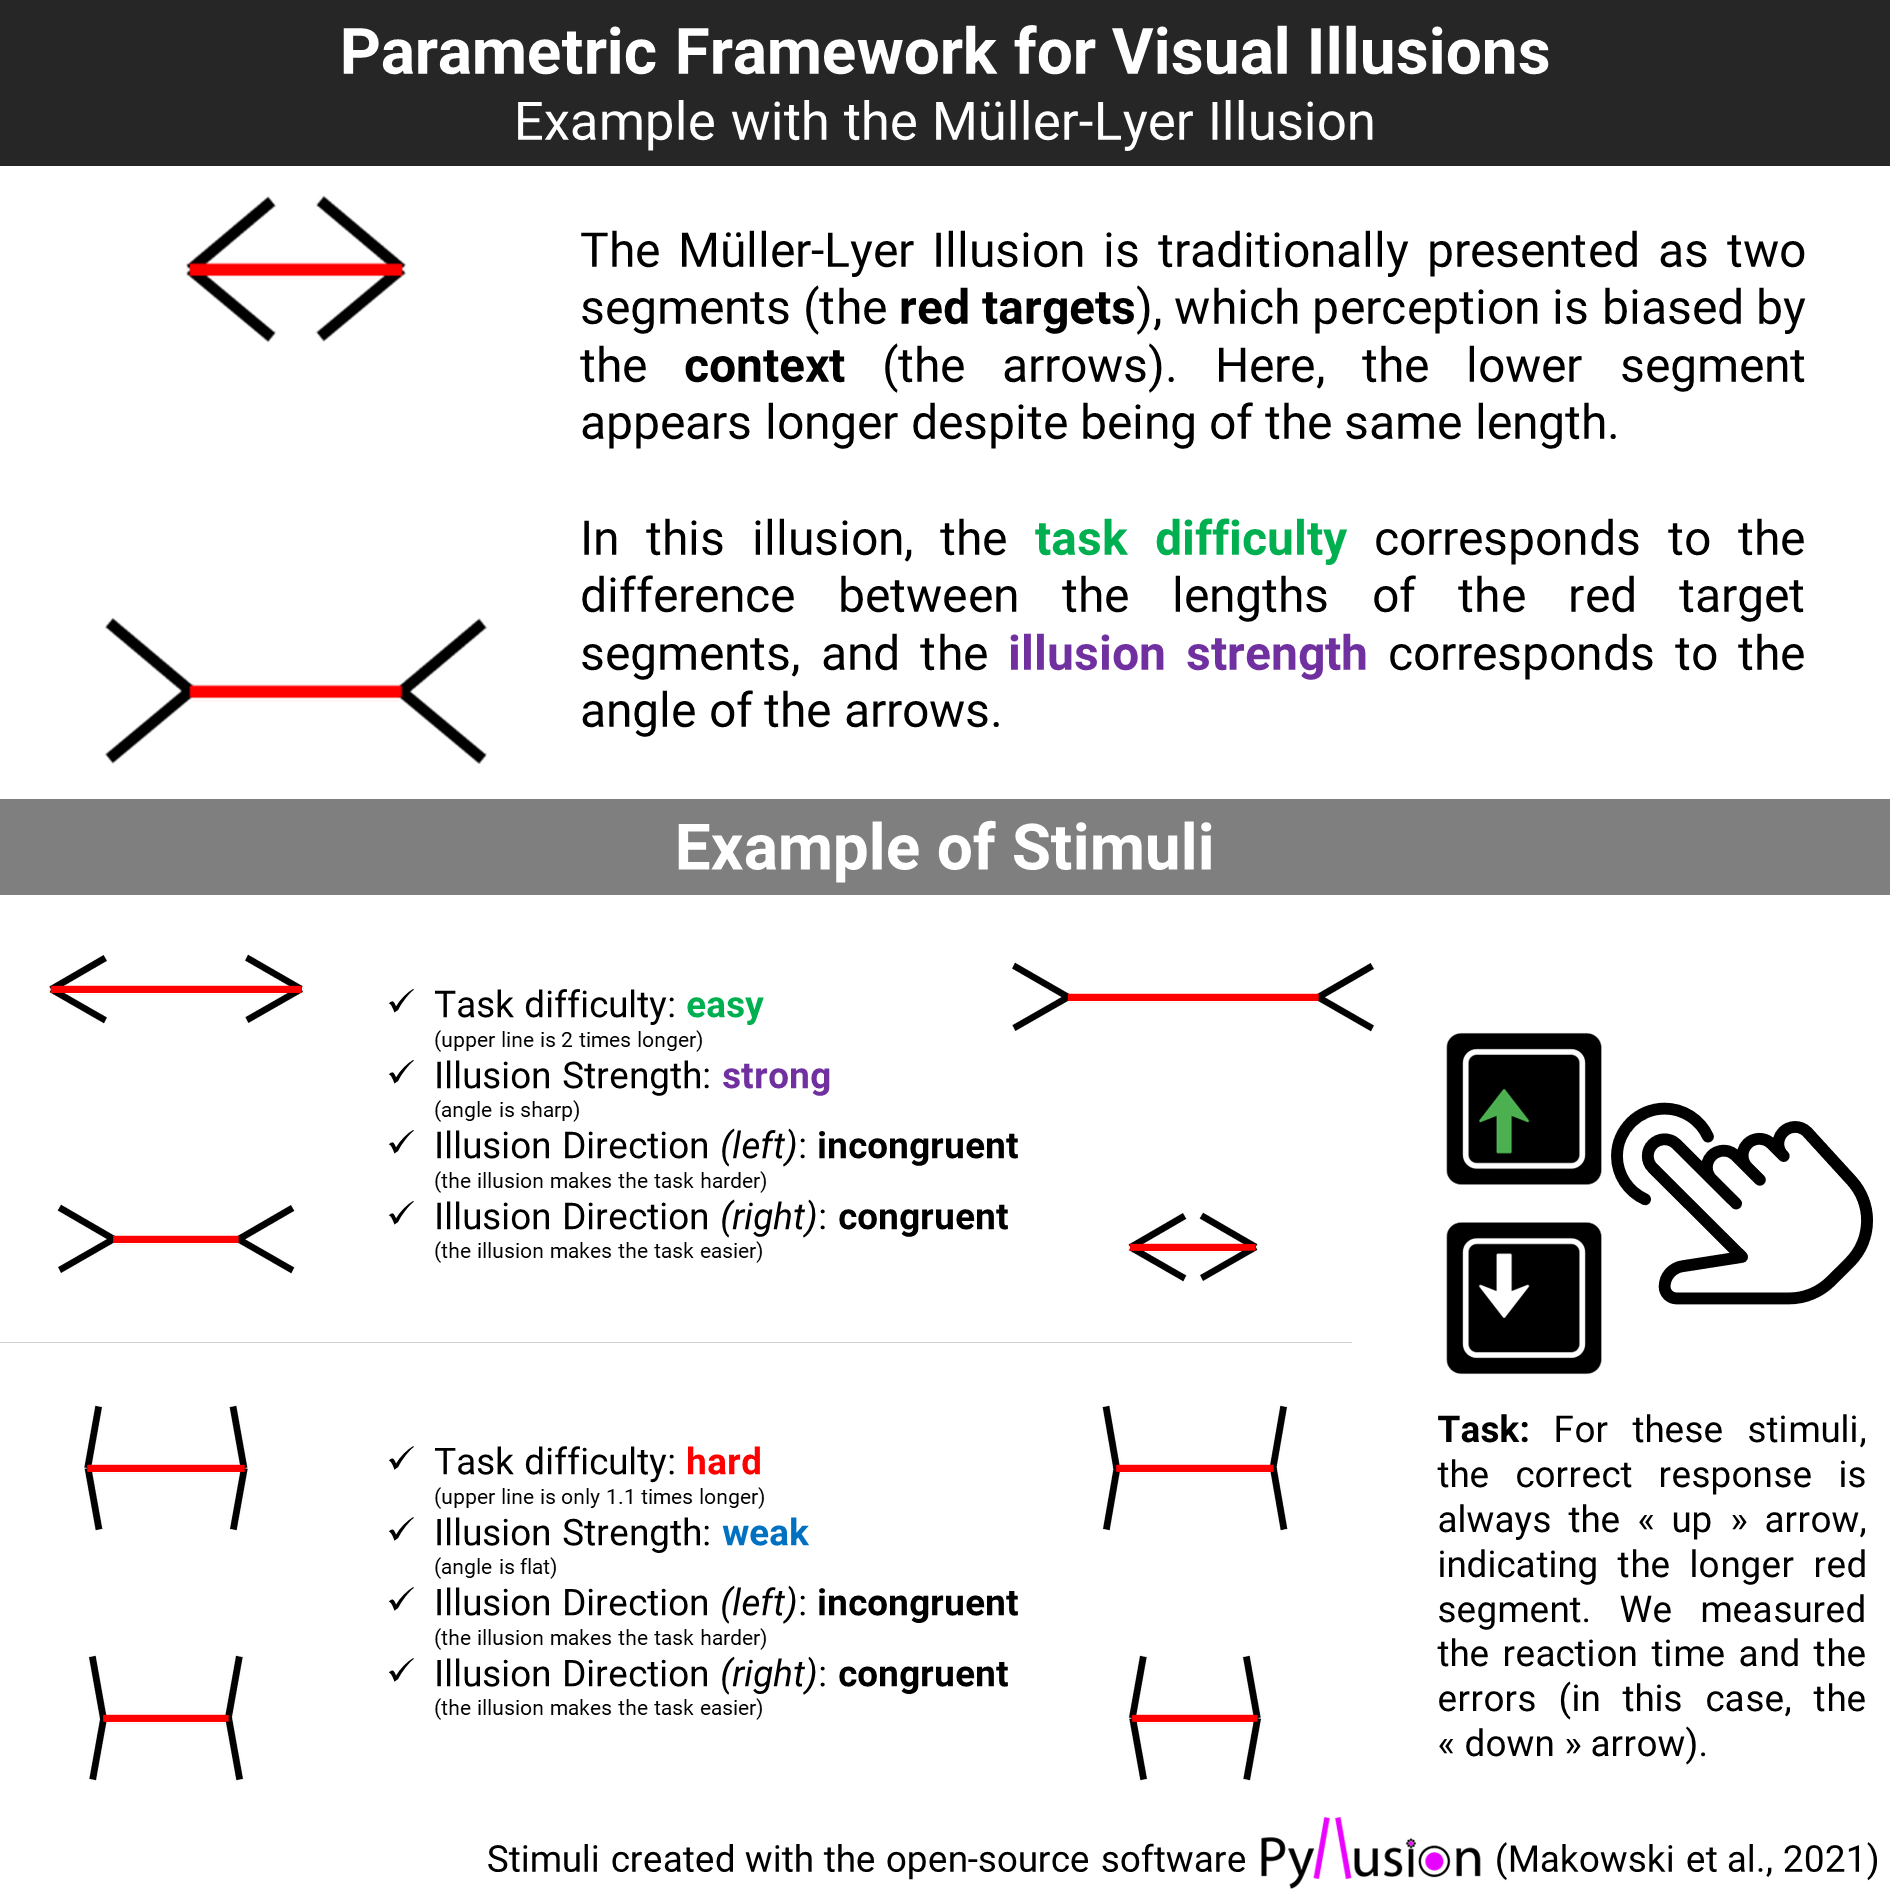
\includegraphics[width=4.2in]{figures/Figure1} \caption{The parametric framework for visual illusions (Makowski et al., 2021) applied to the Müller-Lyer illusion (above). Below are examples of stimuli showcasing the manipulation of two parameters, task difficulty and illusion strength.}\label{fig:unnamed-chunk-2}
\end{figure}

Indeed, many visual illusions can be seen as being composed of \emph{targets} (e.g., same-length lines), of which perception is biased by the \emph{context} (e.g., in the Müller-Lyer illusion, the same-length line segments appear to have different lengths when they end with inwards or outwards pointing arrows).
Past illusion studies traditionally employed paradigms focusing on participants' subjective experience, by asking them to what extent they perceive two identical targets as different (\emph{REF}), or having them adjust the targets to a reference stimulus relying only on their perception (Grzeczkowski et al., 2018; Mylniec \& Bednarek, 2016a). Alternatively, \emph{Pyllusions} allows the creation of illusions in which the targets are objectively different (e.g., one segment is truly more or less longer than the other), and in which the illusion varies in strength (the biasing angle of the arrows is more or less acute).

This opens the door for an experimental task in which participants have to make perceptual judgments about the targets (e.g., which segment in the longest) under different conditions of objective difficulty and illusion strength. Moreover, the illusion effect can be either ``incongruent'' (making the task even harder by biasing the perception in the opposite way) or ``congruent'' (making the task easier). Although visual illusions are inherently tied to subjective perception, this framework allows a reversal of the traditional paradigm to potentially quantify the ``objective'' effect of illusions by measuring its behavioral effect (error rate and reaction times) on the performance in a perceptual task.

In the present set of preregistered studies, we will first test this novel paradigm by investigating if the effect of illusion and task difficulty can be manipulated continuously, and separated statistically. Then, we will further utilize the paradigm to assess whether 10 different classic illusions (Delboeuf, Ebbinghaus, Rod and Frame, Vertical-Horizontal, Zöllner, White, Müller-Lyer, Ponzo, Poggendorff, Contrast) share a common latent factor. Finally, we will investigate how the the inter-individual sensitivity to illusions relates to dispositional variables, such as demographic characteristics and personality.

In line with total open-science standards, all the material (stimuli generation code, experiment code, raw data, analysis script with complementary figures and analyses, preregistration, etc.) is available at \href{https://github.com/RealityBending/IllusionGameValidation}{\textbf{https://github.com/RealityBending/IllusionGameValidation}}.

\hypertarget{study-1}{%
\section{Study 1}\label{study-1}}

\hypertarget{aim}{%
\subsection{Aim}\label{aim}}

Study 1 can be seen as a pilot experiment aiming to gather some preliminary data to assess if the stimuli generated by \emph{Pyllusion} behaves as expected for each of the 10 illusion types (i.e., whether an increase of task difficulty and illusion strength leads to an increase of errors); and develop an intuition about the magnitude of effects, to refine the stimuli parameters to a more sensible range (i.e., not overly easy and not impossibly hard) for the next study.

\hypertarget{procedure}{%
\subsection{Procedure}\label{procedure}}

We generated 56 stimuli for each of the 10 illusion types. These stimuli resulted from the combination of 8 linearly-spread levels levels of task difficulty (e.g., {[}1, 2, 3, 4, 5, 6, 7{]}, where 1 corresponds to the higher difficulty - i.e., the smallest objective difference between targets) and 7 levels of illusion strength (3 values of strength on the congruent side, 3 on the incongruent side, and 0; e.g., {[}-3, -2, -1, 0, 1, 2, 3{]}, where negative values correspond to congruent illusion strengths).

The 10 illusion blocks were randomly presented, and the order of the 56 stimuli within the blocks was also randomized. After the first series of 10 blocks, another series was done (with new randomized order of blocks and trials). In total, each participant saw 56 different trials per 10 illusion type, repeated 2 times (total = 1120 trials), to which they had to respond ``as fast as possible without making errors'' (i.e., an explicit double constraint to mitigate the inter-individual variability in the speed-accuracy trade off). The task was implemented using \emph{jsPsych} (De Leeuw, 2015). The instructions for each illusion type are available in the experiment code.

\hypertarget{participants}{%
\subsection{Participants}\label{participants}}

Fifty-two participants were recruited via \emph{Prolific} (\url{www.prolificacademic.co.uk}), a crowd-sourcing platform providing high data quality (Peer et al., 2022). The only inclusion criterion was a fluent proficiency in English to ensure that the task instructions would be well-understood. Participants were incentivised with a reward of about \textsterling 7.5 for completing the task, which took about 50 minutes to finish.

We removed 6 participants upon inspection of the average error rage (when close to 50\%, suggesting random answers), and when the reaction time distribution was implausibly fast. For the remaining participants, we discarded blocks where the error rate was higher than 50\% (possibly indicating that instructions got misunderstood; e.g., participants were selecting the shorter line instead of the longer one). Finally, we removed 692 (1.37\%) trials based on an implausibly short or long response time (\textless{} 150 ms or \textgreater{} 3000 ms).

The final sample included 46 participants (Mean age = 26.7, SD = 7.7, range: {[}19, 60{]}; Sex: 39.1\% females, 56.5\% males).

\hypertarget{data-analysis}{%
\subsection{Data Analysis}\label{data-analysis}}

The analysis of study 1 focused on the probability of errors as the main outcome variable. For each illusion, we started by visualizing the average effect of task difficulty and illusion strength to gain some intuition on the underlying generative model. Next, we tested the performance of various logistic models differing in their specifications, such as: with or without a transformation of the task difficulty (log, square root or cubic root), with or without a 2nd order polynomial term for the illusion strength, and with or without the illusion side (up \emph{vs.} down or left \emph{vs.} right) as an additional predictor. We then fitted the best performing model under a Bayesian framework, and compared its visualization with that of a General Additive Model (GAM), which has an increased ability of mapping underlying potentially non-linear relationships (at the expense of model simplicity).

The analysis was carried out using \emph{R 4.2} (R Core Team, 2022), \emph{brms} (Bürkner, 2017), the \emph{tidyverse} (Wickham et al., 2019), and the \emph{easystats} collection of packages (Lüdecke et al., 2021, 2019; Makowski et al., 2020, 2019).

\hypertarget{results}{%
\subsection{Results}\label{results}}

The statistical models suggested that the effect of task difficulty had a cubic relationship with error rate for the Delboeuf and Ebbinghaus illusions (both composed of circular shapes), square relationship for the Rod and Frame and Vertical-Horizontal illusions, cubic relationship for the Zöllner and Poggendorff illusions, exponential relationship for the White illusion, cubic relationship for the Müller-Lyer and Ponzo illusions (both based on line lengths), and linear relationship for the Contrast illusion. All models suggested a significant effect of illusion strength and task difficulty. See details and figures in the analysis script.

\hypertarget{discussion}{%
\subsection{Discussion}\label{discussion}}

This study provided a clearer understanding of the magnitude of the parametric effects at stake and the type of interaction between them. Furthermore, it allowed us to better understand and test the stimuli generated by \emph{Pyllusion}, as well as uncover technical bugs and issues (for instance, the specification direction of the illusion strength was reversed for a few illusions), which were fixed by a new software release. Crucially, this study allowed us to refine the range of task difficulty and illusion strength values in order to maximize information gain.

In most illusions, the task difficulty exhibited monotonic power-law scaled effects, which is in line with the psychophysics literature on perceptual decisions (Bogacz et al., 2006; Ditzinger, 2010; Shekhar \& Rahnev, 2021). One notable result was the illusion effect pattern for the Zöllner illusion, which suggested a non-linear relationship. By generating a wider range of illusion strength values, the next study will attempt at clarifying this point.

\hypertarget{study-2}{%
\section{Study 2}\label{study-2}}

\hypertarget{aim-1}{%
\subsection{Aim}\label{aim-1}}

The aim of study 2 was two-fold. In the first part, we carefully modeled the error rate and the reaction time of each illusion type in order to validate our novel paradigm and show that the effect of illusions can be manipulated continuously. In the second part, we derived the participant-level scores from the models (i.e., the effect of illusion strength for each individual) and analyzed their latent factors structure.

\hypertarget{procedure-1}{%
\subsection{Procedure}\label{procedure-1}}

The paradigm of study 2 was similar to that of study 1, with the following changes. The illusory stimuli were re-generated within a refined space of parameters based on the results of study 1. Moreover, taking into account the findings of study 1, we used non-linearly spaced difficulty levels, depending on the best underlying model (i.e., with an exponential, square or cubic spacing depending on the relationship). For instance, a linear space of {[}0.1, 0.4, 0.7, 1.0{]} can be transformed to an exponential space of {[}0.1, 0.34, 0.64, 1.0{]}.

Additionally, instead of repeating each stimulus two times, we generated illusions using more levels of difficulty and illusion strength. As such, for each illusion type, we generated a total of 134 stimuli that were split into two groups (67 stimuli per illusion block). Furthermore, instead of a simple break screen, we added two personality questionnaires between the two series of 10 illusion blocks (see study 3).

\hypertarget{participants-1}{%
\subsection{Participants}\label{participants-1}}

Using the same recruitment procedure as in study 1, we recruited 256 participants, out of which 6 were identified as outliers and excluded, leaving a final sample of 250 participants (Mean age = 26.5, SD = 7.6, range: {[}18, 69{]}; Sex: 48\% females, 52\% males). Please see study 3 for the full demographic breakdown. We discarded blocks with more than 50\% of errors (2.16\% of trials) and 0.76\% trials with extreme response times (\textless{} 125 ms or \textgreater{} 4 SD above mean).

\hypertarget{data-analysis-1}{%
\subsection{Data Analysis}\label{data-analysis-1}}

The first part of the analysis focused on modelling the effect of illusion strength and task difficulty on errors and reaction time (RT), within each illusion. In order to achieve that, we started by fitting General Additive Models (GAMs), which can accommodate possible non-linear effects and interactions. Errors were analyzed using Bayesian logistic mixed models, and RTs of correct responses were analyzed using an ex-Gaussian family with the same fixed effects entered for the location \(\mu\) (mean), scale \(\sigma\) (spread) and tail-dominance \(\tau\) of the RT distribution (Balota \& Yap, 2011; Matzke \& Wagenmakers, 2009).

Using the GAMs as a ``ground-truth'', we attempted at approximating them using general linear models, which have the advantage of estimating the participant-level variability of the effects (via random slopes). Following a comparison of models with a combination of transformations (raw, log, square root or cubic root) on the main predictors (task \emph{difficulty} and illusion \emph{strength}), we selected and fitted the best model (best on their indices of fit), and compared their output visually (see \textbf{Figure 2}).

We then extracted the inter-individual variability in the effect of illusion strength and its interaction with task difficulty, and used it as participant-level scores. Finally, We explored the relationship of these indices across different illusions using exploratory factor analysis (EFA) and structural equation modelling (SEM).

\hypertarget{results-1}{%
\subsection{Results}\label{results-1}}

The best models were \(log(diff)*strength\) for Delboeuf; \(sqrt(diff)*strength\) for Ebbinghaus; \(log(diff)*log(strength)\) for Rod and Frame; \(sqrt(diff)*sqrt(strength)\) for Vertical-Horizontal; \(cbrt(diff)*strength\) for Zöllner; \(diff*sqrt(strength)\) and \(log(diff)*strength\) respectively for errors and RT in White; \(sqrt(diff)*sqrt(strength)\) and \(sqrt(diff)*strength\) respectively for errors and RT in Müller-Lyer; \(cbrt(diff)*strength\) for Ponzo; \(cbrt(diff)*sqrt(strength)\) and \(cbrt(diff)*strength\) respectively for errors and RT in Poggendorff; \(sqrt(diff)*sqrt(strength)\) for Contrast. In all of these models, the effects of illusion strength, task difficulty and their interaction were significant.

For errors, most of the models closely matched their GAMs counterpart (see \textbf{Figure 2}), with the exception of Delboeuf (for which the GAM suggested a non-monotonic effect of illusion strength with a local minimum at 0) and Zöllner, in which theoretically congruent illusion effects were related to increased error rate.

\begin{figure}
\includegraphics[width=20in]{figures/Figure2} \caption{CAPTION.}\label{fig:unnamed-chunk-3}
\end{figure}

For RTs, the GAMs suggested a consistent non-linear relationship between RT and illusion strength: as the illusion strength increase beyond a certain threshold, the participants respond faster. While this is is not surprising (strong illusions are likely so effective in biasing perception that it is ``easier'', i.e., faster, to make the wrong decision), the linear models were not designed to capture this - likely quadratic - pattern and hence are not good representatives of the underlying dynamics. As such, we decided not to use them for the individual scores analysis.

Though imperfect, we believe that the random-slope models capture inter-individual differences with more accuracy (and are also more conservative estimates due shrinkage) than basic empirical scores, such as the total number of errors, or the average RT. Thus, for each illusion and within each participant, we extracted the effect of illusion strength and its interaction with task difficulty when the illusion effect was incongruent. These twenty participant-level scores were subjected to exploratory factor analysis (EFA). The Method Agreement Procedure (Lüdecke et al., 2020) suggested the presence of 7 latent factors. An oblique (\emph{oblimin} rotation) factor solution explaining 66.69\% of variance suggested separate dimensions for the effect of Zöllner, White, Poggendorff, Contrast, Ebbinghaus, Delboeuf, and a common factor for the parameters related to Müller-Lyer, Vertical-Horizontal, Ponzo and Rod and Frame. We submitted these factors to a second-level analysis and extracted two orthogonal (\emph{varimax} rotation) factors. The first factor was loaded by all the previous dimensions with the exception of Delboeuf, which formed its own separate factor.

Finally, we tested this data-driven model (\emph{m0}) against four other structural models using structural equation modelling (SEM): one in which the two parameters of each of the 10 illusions (illusion strength and interaction with task difficulty) loaded on separate factors, which then all loaded on a common factor (\emph{m1}); one which the parameters were grouped by illusion type (lines, circles, contrast and angle) before loading on a common factor (\emph{m2}); one in which all the parameters related to strength, and all the parameters related to the interaction loaded onto two respective factors, which then loaded on a common factor (\emph{m3}); and one in which there was no intermediate level: all 20 parameters loaded directly on a common factor (\emph{m4}).

The model \emph{m1}, in which the parameters loaded on a first level of 10 illusion-specific factors, which then all loaded on a common factor significantly outperformed the other models. Its indices of fit were ranging from acceptable to satisfactory (CFI = .92; SRMR = .08; NNFI = .91; PNFI = .74; RMSEA = .08), and all the specified effects were significant. The illusion-specific latent factors were loaded positively by the sensitivity to illusion strength, and positively by the interaction effect with task difficulty (with the exception of Delboeuf, Ebbinghaus, Vertical-Horizontal, Müller-Lyer and Contrast, for which the loading was negative). The general factor of illusion sensitivity, labelled Factor \emph{i} (i- for illusion), explained 48.02\% of the total variance of the initial dataset, and was strongly related to Vertical-Horizontal (\(\beta_{std.}=0.83\)), Müller-Lyer (\(\beta_{std.}=0.76\)), Ponzo (\(\beta_{std.}=0.65\)), Ebbinghaus (\(\beta_{std.}=0.64\)); moderately to Zöllner (\(\beta_{std.}=0.53\)), Poggendorff (\(\beta_{std.}=0.44\)), Rod and Frame (\(\beta_{std.}=0.42\)), Contrast (\(\beta_{std.}=0.40\)) and White (\(\beta_{std.}=0.35\)); and weakly to Delboeuf (\(\beta_{std.}=0.19\)). We then computed, for each participant, its score for the 10 illusion-specific factors and for the general Factor \emph{i}.

We have to keep in mind that these individual scores are the result of several layers of simplification: 1) the individual coefficient is that of simpler models that sometimes do not perfectly capture the underlying dynamics (especially in the case of Delboeuf and Zöllner); 2) we only used the models on error rate, which could be biased by the speed-accuracy decision criterion used by participants; 3) the structural equation model used to compute the scores also incorporated multiple levels of abstractions. Thus, in order to validate the individual scores, we computed the correlation between them and simple empirical scores, such as the average error rate and the mean RT in the task. This analysis revealed strong and significant correlations between each illusion-specific factor and the average amount of errors in its respective task. Moreover, each individual score was strongly associated with the average RT across multiple illusion types. This suggests that the individual scores obtained from the structural equation model do capture the sensitivity of each participant to visual illusions, manifesting in both the amount of errors and high reaction times.

\hypertarget{discussion-1}{%
\subsection{Discussion}\label{discussion-1}}

This study confirmed that it was possible to continuously manipulate the effect of illusion strength for 10 classical illusions. Increasing the illusion strength increased the likelihood of errors, as well as the average and spread of RTs (but only up to a point, after which participants become faster at responding with the wrong answer). Future studies are needed to explore reaction times and try to identify the most appropriate models, and / or use models that integrate errors and reaction time (e.g., drift diffusion models).

The effect on errors was monotonic for most illusions, with the exception of Delboeuf and Zöllner. For both of them, mildly congruent illusion strengths (which theoretically were supposed to be associated with less errors than incongruent effects) were related to a small and strong increase of errors, respectively. For Delboeuf, we believe that it was an artifact caused by illusion generation algorithm: the outline of the target circles was always created as slightly bigger, which made the difference between them more obvious at an illusion strength of 0. This was fixed in latest release of \emph{Pyllusion} (v1.2), which now generate outlines of the same size as the target circle. For Zöllner, however, we did not find a good explanation of the pattern. \textbf{TODO: is there some explanation that we can find in the literature?}

Finally, this study provided evidence for both the existence of illusion-specific factors, as well as for a common latent factor (labelled Factor \emph{i}) that explained about half of the total variance. These participant-level scores were related to the error rate and average reaction time, and can thus be interpreted as indices of illusion sensitivity.

\hypertarget{study-3}{%
\section{Study 3}\label{study-3}}

\hypertarget{aim-2}{%
\subsection{Aim}\label{aim-2}}

Study 3 aimed at investigating the links between the inter-individual scores of illusion sensitivity (obtained in study 2), and demographic and dispositional variables.

\hypertarget{procedure-2}{%
\subsection{Procedure}\label{procedure-2}}

This study was based on the data collected in study 2. The variables of interest here were taken from the questionnaires that were inserted in between the two series of illusion blocks. We used the \emph{IPIP6} (24 items, Sibley et al., 2011) to measure 6 ``normal'' personality traits (Extraversion, Openness, Conscientiousness, Agreeableness, Neuroticism and Honesty-humility), and the PID-5 (25 items, Hopwood et al., 2012) to measure ``pathological'' personality traits (Disinhibition, Antagonism, Detachment, Negative Affect and Psychoticism). The participants were the same as in study 2 (see \textbf{Figure 3}). However, due to a technical issue, no personality data was recorded for the first eight participants.

\begin{figure}
\includegraphics[width=20in]{figures/Figure2} \caption{CAPTION.}\label{fig:unnamed-chunk-4}
\end{figure}

\hypertarget{data-analysis-2}{%
\subsection{Data Analysis}\label{data-analysis-2}}

\hypertarget{results-2}{%
\subsection{Results}\label{results-2}}

\hypertarget{discussion-2}{%
\subsection{Discussion}\label{discussion-2}}

\hypertarget{general-discussion}{%
\section{General Discussion}\label{general-discussion}}

Using the parametric illusion generation framework we developed, Pyllusion (Makowski et al., 2021b), we have hence shown that illusions can be manipulated continuously across several different visual illusions. This opens the door for new illusions-based paradigms and tasks, therefore making it possible for future researchers to directly manipulate specific features and parameters of the illusion that are of interest. The validation of this novel framework also affords future illusion scientists a standardized measure of illusion susceptibility, instead of relying on conventional methods that depend upon participants' subjective perceptions. In our paradigm, in which we apply this approach to a reaction-time task, we were able to measure inter-individual scores of objective illusion sensitivity.

Most notably, there is currently no universally agreed upon neurocognitive mechanism that explains individuals' susceptibility to visual illusions (Mylniec \& Bednarek, 2016b). For instance, while some researchers have tried to explain our sensitivity to illusory effects as a result of deficits in the low-level visual processing system (Cretenoud et al., 2019b; Gori et al., 2016), others have provided a compelling case using a top-down approach, suggesting that such visual phenomena occur as a result of a conflict between our visual input and our prior beliefs(Caporuscio et al., 2022; Teufel et al., 2018a).

Furthermore, results from studies that have been conducted to elucidate the mechanism underlying our susceptibility towards visual illusions remain relatively mixed. Whereas higher resistance towards such illusions have been reported for individuals with pathologically strong prior beliefs (such as schizophrenics) and atypical sensory perception (for example, those with autism spectrum disorder {[}ASD{]}) (Giaouri \& Alevriadou, 2011; Keane et al., 2014; Notredame et al., 2014; Park et al., 2022), other studies have found no significant differences between such individuals and healthy controls (Kaliuzhna et al., 2019; Spencer \& Ghorashi, 2014; Tibber et al., 2013; Yang et al., 2012) or only a weak correlation between the magnitude of visual illusions and such individuals' susceptibility to these illusory effects (Grzeczkowski et al., 2018; Manning et al., 2017).

\hypertarget{future-directions}{%
\section{Future Directions}\label{future-directions}}

We strongly invite researchers to explore and re-analyze our dataset with other approaches and methods to push the understanding of visual illusions and illusion sensitivity further. The task, data and analysis script are available in open-access at \href{https://github.com/RealityBending/IllusionGameValidation}{\textbf{https://github.com/RealityBending/IllusionGameValidation}}.

\hypertarget{acknowledgments}{%
\section{Acknowledgments}\label{acknowledgments}}

We would like to thank Tam Pham and Zen J. Lau for their contribution to \emph{Pyllusion}, as well as Prof Dólos for the inspiration.

\newpage

\hypertarget{references}{%
\section{References}\label{references}}

\hypertarget{refs}{}
\begin{CSLReferences}{1}{0}
\leavevmode\vadjust pre{\hypertarget{ref-balota2011moving}{}}%
Balota, D. A., \& Yap, M. J. (2011). Moving beyond the mean in studies of mental chronometry: The power of response time distributional analyses. \emph{Current Directions in Psychological Science}, \emph{20}(3), 160--166.

\leavevmode\vadjust pre{\hypertarget{ref-bogacz2006}{}}%
Bogacz, R., Brown, E., Moehlis, J., Holmes, P., \& Cohen, J. D. (2006). The physics of optimal decision making: A formal analysis of models of performance in two-alternative forced-choice tasks. \emph{Psychological Review}, \emph{113}(4), 700--765. \url{https://doi.org/10.1037/0033-295X.113.4.700}

\leavevmode\vadjust pre{\hypertarget{ref-Burkner2017}{}}%
Bürkner, P.-C. (2017). {brms}: An {R} package for {Bayesian} multilevel models using {Stan}. \emph{Journal of Statistical Software}, \emph{80}(1), 1--28. \url{https://doi.org/10.18637/jss.v080.i01}

\leavevmode\vadjust pre{\hypertarget{ref-caporuscio2022}{}}%
Caporuscio, C., Fink, S. B., Sterzer, P., \& Martin, J. M. (2022). When seeing is not believing: A mechanistic basis for predictive divergence. \emph{Consciousness and Cognition}, \emph{102}, 103334. \url{https://doi.org/10.1016/j.concog.2022.103334}

\leavevmode\vadjust pre{\hypertarget{ref-carbon2014}{}}%
Carbon, C.-C. (2014). Understanding human perception by human-made illusions. \emph{Frontiers in Human Neuroscience}, \emph{8}. \url{https://www.frontiersin.org/articles/10.3389/fnhum.2014.00566}

\leavevmode\vadjust pre{\hypertarget{ref-cretenoud2020}{}}%
Cretenoud, A. F., Francis, G., \& Herzog, M. H. (2020). When illusions merge. \emph{Journal of Vision}, \emph{20}(8), 12. \url{https://doi.org/10.1167/jov.20.8.12}

\leavevmode\vadjust pre{\hypertarget{ref-cretenoud2019}{}}%
Cretenoud, A. F., Karimpur, H., Grzeczkowski, L., Francis, G., Hamburger, K., \& Herzog, M. H. (2019b). Factors underlying visual illusions are illusion-specific but not feature-specific. \emph{Journal of Vision}, \emph{19}(14), 12. \url{https://doi.org/10.1167/19.14.12}

\leavevmode\vadjust pre{\hypertarget{ref-cretenoud2019a}{}}%
Cretenoud, A. F., Karimpur, H., Grzeczkowski, L., Francis, G., Hamburger, K., \& Herzog, M. H. (2019a). Factors underlying visual illusions are illusion-specific but not feature-specific. \emph{Journal of Vision}, \emph{19}(14), 12. \url{https://doi.org/10.1167/19.14.12}

\leavevmode\vadjust pre{\hypertarget{ref-day1972}{}}%
Day, R. H. (1972). Visual Spatial Illusions: A General Explanation: A wide range of visual illusions, including geometrical distortions, can be explained by a single principle. \emph{Science}, \emph{175}(4028), 1335--1340. \url{https://doi.org/10.1126/science.175.4028.1335}

\leavevmode\vadjust pre{\hypertarget{ref-de2015jspsych}{}}%
De Leeuw, J. R. (2015). jsPsych: A JavaScript library for creating behavioral experiments in a web browser. \emph{Behavior Research Methods}, \emph{47}(1), 1--12.

\leavevmode\vadjust pre{\hypertarget{ref-ditzinger2010}{}}%
Ditzinger, T. (2010). \emph{Optical illusions: Examples for nonlinear dynamics in perception} (Vol. 328, pp. 179--191).

\leavevmode\vadjust pre{\hypertarget{ref-eagleman2001}{}}%
Eagleman, D. M. (2001). Visual illusions and neurobiology. \emph{Nature Reviews Neuroscience}, \emph{2}(12), 920--926. \url{https://doi.org/10.1038/35104092}

\leavevmode\vadjust pre{\hypertarget{ref-giaouri2011}{}}%
Giaouri, S., \& Alevriadou, A. (2011). Are children with down syndrome susceptible to visual illusions? \emph{Procedia - Social and Behavioral Sciences}, \emph{15}, 1988--1992. \url{https://doi.org/10.1016/j.sbspro.2011.04.040}

\leavevmode\vadjust pre{\hypertarget{ref-gomez-villa2022}{}}%
Gomez-Villa, A., Martín, A., Vazquez-Corral, J., Bertalmío, M., \& Malo, J. (2022). On the synthesis of visual illusions using deep generative models. \emph{Journal of Vision}, \emph{22}(8), 2. \url{https://doi.org/10.1167/jov.22.8.2}

\leavevmode\vadjust pre{\hypertarget{ref-gori2016}{}}%
Gori, S., Molteni, M., \& Facoetti, A. (2016). Visual illusions: An interesting tool to investigate developmental dyslexia and autism spectrum disorder. \emph{Frontiers in Human Neuroscience}, \emph{10}, 175. \url{https://doi.org/10.3389/fnhum.2016.00175}

\leavevmode\vadjust pre{\hypertarget{ref-grzeczkowski2018}{}}%
Grzeczkowski, L., Roinishvili, M., Chkonia, E., Brand, A., Mast, F. W., Herzog, M. H., \& Shaqiri, A. (2018). Is the perception of illusions abnormal in schizophrenia? \emph{Psychiatry Research}, \emph{270}, 929--939. \url{https://doi.org/10.1016/j.psychres.2018.10.063}

\leavevmode\vadjust pre{\hypertarget{ref-hamburger2016}{}}%
Hamburger, K. (2016). Visual Illusions Based on Processes: New Classification System Needed: \emph{Perception}. \url{https://doi.org/10.1177/0301006616629038}

\leavevmode\vadjust pre{\hypertarget{ref-hopwood2012}{}}%
Hopwood, C. J., Thomas, K. M., Markon, K. E., Wright, A. G. C., \& Krueger, R. F. (2012). DSM-5 personality traits and DSM{\textendash}IV personality disorders. \emph{Journal of Abnormal Psychology}, \emph{121}(2), 424--432. \url{https://doi.org/10.1037/a0026656}

\leavevmode\vadjust pre{\hypertarget{ref-kaliuzhna2019}{}}%
Kaliuzhna, M., Stein, T., Rusch, T., Sekutowicz, M., Sterzer, P., \& Seymour, K. J. (2019). No evidence for abnormal priors in early vision in schizophrenia. \emph{Schizophrenia Research}, \emph{210}, 245--254. \url{https://doi.org/10.1016/j.schres.2018.12.027}

\leavevmode\vadjust pre{\hypertarget{ref-keane2014}{}}%
Keane, B. P., Joseph, J., \& Silverstein, S. M. (2014). Late, not early, stages of Kanizsa shape perception are compromised in schizophrenia. \emph{Neuropsychologia}, \emph{56}, 302--311. \url{https://doi.org/10.1016/j.neuropsychologia.2014.02.001}

\leavevmode\vadjust pre{\hypertarget{ref-lamme2020}{}}%
Lamme, V. A. F. (2020). Visual functions generating conscious seeing. \emph{Frontiers in Psychology}, \emph{11}. \url{https://www.frontiersin.org/articles/10.3389/fpsyg.2020.00083}

\leavevmode\vadjust pre{\hypertarget{ref-parametersArticle}{}}%
Lüdecke, D., Ben-Shachar, M., Patil, I., \& Makowski, D. (2020). Extracting, computing and exploring the parameters of statistical models using {R}. \emph{Journal of Open Source Software}, \emph{5}(53), 2445. \url{https://doi.org/10.21105/joss.02445}

\leavevmode\vadjust pre{\hypertarget{ref-performanceArticle}{}}%
Lüdecke, D., Ben-Shachar, M., Patil, I., Waggoner, P., \& Makowski, D. (2021). {performance}: An {R} package for assessment, comparison and testing of statistical models. \emph{Journal of Open Source Software}, \emph{6}(60), 3139. \url{https://doi.org/10.21105/joss.03139}

\leavevmode\vadjust pre{\hypertarget{ref-insightArticle}{}}%
Lüdecke, D., Waggoner, P., \& Makowski, D. (2019). Insight: A unified interface to access information from model objects in {R}. \emph{Journal of Open Source Software}, \emph{4}(38), 1412. \url{https://doi.org/10.21105/joss.01412}

\leavevmode\vadjust pre{\hypertarget{ref-bayestestRArticle}{}}%
Makowski, D., Ben-Shachar, M., \& Lüdecke, D. (2019). {bayestestR}: Describing effects and their uncertainty, existence and significance within the {Bayesian} framework. \emph{Journal of Open Source Software}, \emph{4}(40), 1541. \url{https://doi.org/10.21105/joss.01541}

\leavevmode\vadjust pre{\hypertarget{ref-correlationArticle}{}}%
Makowski, D., Ben-Shachar, M., Patil, I., \& Lüdecke, D. (2020). Methods and algorithms for correlation analysis in {R}. \emph{Journal of Open Source Software}, \emph{5}(51), 2306. \url{https://doi.org/10.21105/joss.02306}

\leavevmode\vadjust pre{\hypertarget{ref-makowski2021}{}}%
Makowski, D., Lau, Z. J., Pham, T., Paul Boyce, W., \& Annabel Chen, S. H. (2021a). A Parametric Framework to Generate Visual Illusions Using Python. \emph{Perception}, \emph{50}(11), 950--965. \url{https://doi.org/10.1177/03010066211057347}

\leavevmode\vadjust pre{\hypertarget{ref-makowski2021a}{}}%
Makowski, D., Lau, Z. J., Pham, T., Paul Boyce, W., \& Annabel Chen, S. H. (2021b). A Parametric Framework to Generate Visual Illusions Using Python. \emph{Perception}, \emph{50}(11), 950--965. \url{https://doi.org/10.1177/03010066211057347}

\leavevmode\vadjust pre{\hypertarget{ref-manning2017}{}}%
Manning, C., Morgan, M. J., Allen, C. T. W., \& Pellicano, E. (2017). Susceptibility to ebbinghaus and müller-lyer illusions in autistic children: A comparison of three different methods. \emph{Molecular Autism}, \emph{8}(1), 16. \url{https://doi.org/10.1186/s13229-017-0127-y}

\leavevmode\vadjust pre{\hypertarget{ref-matzke2009psychological}{}}%
Matzke, D., \& Wagenmakers, E.-J. (2009). Psychological interpretation of the ex-gaussian and shifted wald parameters: A diffusion model analysis. \emph{Psychonomic Bulletin \& Review}, \emph{16}(5), 798--817.

\leavevmode\vadjust pre{\hypertarget{ref-mylniec2016}{}}%
Mylniec, A., \& Bednarek, H. (2016b). Field dependence, efficiency of information processing in working memory and susceptibility to orientation illusions among architects. \emph{Polish Psychological Bulletin}, \emph{47}(1), 112--122. \url{https://doi.org/10.1515/ppb-2016-0012}

\leavevmode\vadjust pre{\hypertarget{ref-mylniec2016a}{}}%
Mylniec, A., \& Bednarek, H. (2016a). Field dependence, efficiency of information processing in working memory and susceptibility to orientation illusions among architects. \emph{Polish Psychological Bulletin}, \emph{47}(1), 112--122. \url{https://doi.org/10.1515/ppb-2016-0012}

\leavevmode\vadjust pre{\hypertarget{ref-notredame2014}{}}%
Notredame, C.-E., Pins, D., Deneve, S., \& Jardri, R. (2014). What visual illusions teach us about schizophrenia. \emph{Frontiers in Integrative Neuroscience}, \emph{8}, 63. \url{https://doi.org/10.3389/fnint.2014.00063}

\leavevmode\vadjust pre{\hypertarget{ref-park2022}{}}%
Park, S., Zikopoulos, B., \& Yazdanbakhsh, A. (2022). Visual illusion susceptibility in autism: A neural model. \emph{European Journal of Neuroscience}, \emph{56}. \url{https://doi.org/10.1111/ejn.15739}

\leavevmode\vadjust pre{\hypertarget{ref-peer2022}{}}%
Peer, E., Rothschild, D., Gordon, A., Evernden, Z., \& Damer, E. (2022). Data quality of platforms and panels for online behavioral research. \emph{Behavior Research Methods}, \emph{54}(4), 1643--1662. \url{https://doi.org/10.3758/s13428-021-01694-3}

\leavevmode\vadjust pre{\hypertarget{ref-RCoreTeam2022}{}}%
R Core Team. (2022). \emph{R: A language and environment for statistical computing}. R Foundation for Statistical Computing. \url{https://www.R-project.org/}

\leavevmode\vadjust pre{\hypertarget{ref-razeghi2022}{}}%
Razeghi, R., Arsham, S., Movahedi, A., \& Sammaknejad, N. (2022). The effect of visual illusion on performance and quiet eye in autistic children. \emph{Early Child Development and Care}, \emph{192}(5), 807--815. \url{https://doi.org/10.1080/03004430.2020.1802260}

\leavevmode\vadjust pre{\hypertarget{ref-shekhar2021}{}}%
Shekhar, M., \& Rahnev, D. (2021). The nature of metacognitive inefficiency in perceptual decision making. \emph{Psychological Review}, \emph{128}(1), 45--70. \url{https://doi.org/10.1037/rev0000249}

\leavevmode\vadjust pre{\hypertarget{ref-sibley2011}{}}%
Sibley, C., Luyten, N., Wolfman, M., Mobberley, A., Wootton, L. W., Hammond, M., Sengupta, N., Perry, R., West-Newman, T., Wilson, M., McLellan, L., Hoverd, W. J., \& Robertson, A. (2011). The mini-IPIP6: Validation and extension of a short measure of the big-six factors of personality in new zealand. \emph{New Zealand Journal of Psychology}, \emph{40}, 142--159.

\leavevmode\vadjust pre{\hypertarget{ref-spencer2014}{}}%
Spencer, K., \& Ghorashi, S. (2014). Oscillatory dynamics of gestalt perception in schizophrenia revisited. \emph{Frontiers in Psychology}, \emph{5}. \url{https://www.frontiersin.org/articles/10.3389/fpsyg.2014.00068}

\leavevmode\vadjust pre{\hypertarget{ref-teufel2018}{}}%
Teufel, C., Dakin, S. C., \& Fletcher, P. C. (2018a). Prior object-knowledge sharpens properties of early visual feature-detectors. \emph{Scientific Reports}, \emph{8}(1), 10853. \url{https://doi.org/10.1038/s41598-018-28845-5}

\leavevmode\vadjust pre{\hypertarget{ref-teufel2018a}{}}%
Teufel, C., Dakin, S., \& Fletcher, P. (2018b). Prior object-knowledge sharpens properties of early visual feature-detectors. \emph{Scientific Reports}, \emph{8}. \url{https://doi.org/10.1038/s41598-018-28845-5}

\leavevmode\vadjust pre{\hypertarget{ref-teufel2015}{}}%
Teufel, C., Subramaniam, N., Dobler, V., Perez, J., Finnemann, J., Mehta, P. R., Goodyer, I. M., \& Fletcher, P. C. (2015). Shift toward prior knowledge confers a perceptual advantage in early psychosis and psychosis-prone healthy individuals. \emph{Proceedings of the National Academy of Sciences}, \emph{112}(43), 13401--13406. \url{https://doi.org/10.1073/pnas.1503916112}

\leavevmode\vadjust pre{\hypertarget{ref-tibber2013}{}}%
Tibber, M., Anderson, E., Bobin, T., Antonova, E., Seabright, A., Wright, B., Carlin, P., Shergill, S., \& Dakin, S. (2013). Visual surround suppression in schizophrenia. \emph{Frontiers in Psychology}, \emph{4}. \url{https://www.frontiersin.org/articles/10.3389/fpsyg.2013.00088}

\leavevmode\vadjust pre{\hypertarget{ref-wickham2019}{}}%
Wickham, H., Averick, M., Bryan, J., Chang, W., McGowan, L., François, R., Grolemund, G., Hayes, A., Henry, L., Hester, J., Kuhn, M., Pedersen, T., Miller, E., Bache, S., Müller, K., Ooms, J., Robinson, D., Seidel, D., Spinu, V., \ldots{} Yutani, H. (2019). Welcome to the tidyverse. \emph{Journal of Open Source Software}, \emph{4}(43), 1686. \url{https://doi.org/10.21105/joss.01686}

\leavevmode\vadjust pre{\hypertarget{ref-yang2012}{}}%
Yang, E., Tadin, D., Glasser, D. M., Hong, S. W., Blake, R., \& Park, S. (2012). Visual Context Processing in Schizophrenia: \emph{Clinical Psychological Science}. \url{https://doi.org/10.1177/2167702612464618}

\end{CSLReferences}


\clearpage
\renewcommand{\listfigurename}{Figure captions}


\end{document}
